Now we present the results obtained from the experiment described in the previous section. We 
analyze the number of SLA renegotiations performed by each API consumer during the 112 day
period of the experiment, and calculate a set of cumulative distribution functions (CDF). These
CDFs describe the probability of finding an API consumer that experienced a given number of
renegotiation events. Figure~\ref{fig:renegotiation_cdf} illustrates the resulting CDFs.

\begin{figure}
\centering
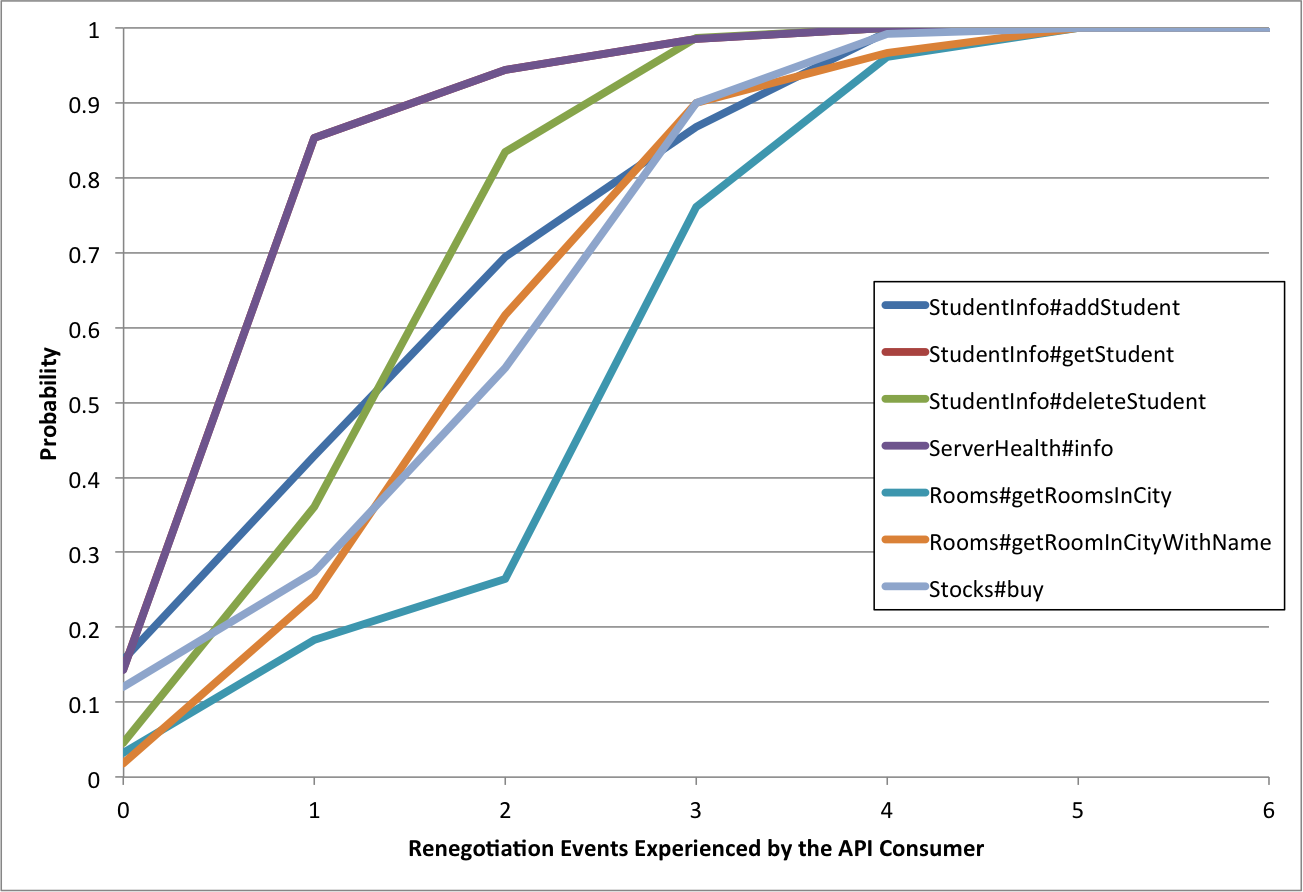
\includegraphics[scale=0.35]{renegotiation_cdf}
\caption{CDF of the number of renegotiation events faced by API consumers.}
\label{fig:renegotiation_cdf}
\vspace{-0.2in}
\end{figure}

According to Figure~\ref{fig:renegotiation_cdf}, the largest number of SLA renegotiations experienced by 
any user is 6. This is
with regard to the StudentInfo\#addStudent operation. Across all web APIs, at least 96\% of the API
consumers experience no more than 4 renegotiation events during the period of 112 days. Further,
at least 76\% of the API consumers see no more than 3 SLA renegotiations, and at least 18\% of
the API consumers observe no more than 1. These statistics
indicate that SLAs predicted by Cerebro for the Google App Engine environment are fairly
stable over time, and renegotiation is required only rarely. From an API consumer's perspective
this is a highly desirable property, since it reduces the frequency and the overhead of SLA renegotiation.

Next we analyze the time duration between SLA renegotiation events. For this we combine the SLA validity
periods computed for each API consumer into a single statistical distribution. 
Table~\ref{tab:validity_periods} shows the 5th percentile, mean and 95th percentile of these combined distributions. 

\begin{table}
\begin{center}
\begin{tabular}{|c|p{1cm}|p{1cm}|p{1cm}|}
\hline
Operation & $5^{th}$ & Mean & $95^{th}$ \\ \hline
StudentInfo\#getStudent & 12.97 & 631.24 & 1911.19 \\ \hline
StudentInfo\#deleteStudent & 7.65 & 472.07 & 2031.59 \\ \hline
StudentInfo\#addStudent & 0.05 & 458.24 & 1711.08 \\ \hline
ServerHealth\#info & 12.96 & 630.01 & 1911.19 \\ \hline
Rooms\#getRoomByName & 8.48 & 345.13 & 1096.53 \\ \hline
Rooms\#getRoomsInCity & 20.56 & 296.44 & 1143.45 \\ \hline
Stocks\#buy & 8.46 & 411.75 & 815.5 \\ \hline
\end{tabular}
\end{center}
\caption{Prediction validity period distributions of different operations in
Google App Engine. $5^{th}$ and $95^{th}$ 
columns represent the 5th and 95th percentiles of the
distributions respectively. All values are in hours.
\label{tab:validity_periods}
}
\end{table}

The smallest
mean SLA validity period observed in our experiments is 296.44 hours (12.35 days). This value is given by the
Rooms\#getRoomsInCity operation. 
This implies that on average, API consumers do not have to renegotiate Cerebro-predicted SLAs
for at least 12.35 days.
The smallest 5th percentile value of 0.05 hours is shown by
the StudentInfo\#addStudent operation, but this appears to be a special case compared to the other web API
operations. The second smallest 5th percentile value of 7.65 hours is shown by the 
StudentInfo\#deleteStudent operation. Therefore, ignoring the StudentInfo\#addStudent operation, API
consumers observe SLA validity periods longer than 7.65 hours at least 95\% of the time. That is, the time
between SLA renegotiations is greater than 7.65 hours at least 95\% of the time.

So far we have simulated the API consumer behavior, assuming that they will be willing to renegotiate the
SLA every time an SLA invalidation occurs in Cerebro. But if the new SLA predicted by Cerebro is very
close to the SLA value that became invalid, the API consumer may not be willing to pay the overhead of
SLA renegotiation. Rather, they would be content to proceed with the old SLA for some more time. In order
to incorporate this behavior of API consumers into our simulation process, we introduce a new parameter 
\textit{sla\_delta\_threshold} into our calculations. This parameter takes on a percentage value which
represents the minimum acceptable percentage difference between the old and new SLA values at renegotiation.
If the percentage difference between the two SLA values is below this threshold, we do not record the
SLA validity period, nor increment the count of the SLA invalidations. In other words, we do not consider
it a renegotiation event at all. We simply carry on with the
old SLA value until we come across an invalidation event, where the new SLA prediction is off from the
old SLA by at least \textit{sla\_delta\_threshold} percent. Note that we can consider our previous experiment
as a special case where \textit{sla\_delta\_threshold} was set to 0.

Next we repeat our simulations with different values for \textit{sla\_delta\_threshold}. Figure~\ref{fig:renegotiation_cdf_sd10}
shows the resulting per-user renegotiation count CDFs when the threshold is set to 10\%. That is, we 
do not prompt the API consumer to renegotiate an SLA, unless the new SLA is at least 10\% off from the old one.
Here we can immediately see that the maximum number of renegotiation events experienced by the API
consumers have dropped to 5 (from 6). Also most of the probabilities have shifted slightly upwards. For instance,
now more than 82\% of the users see 3 or less renegotiation events. Therefore, the introduction of the
\textit{sla\_delta\_threshold} has made renegotiations even more scarce.

\begin{figure}
\centering
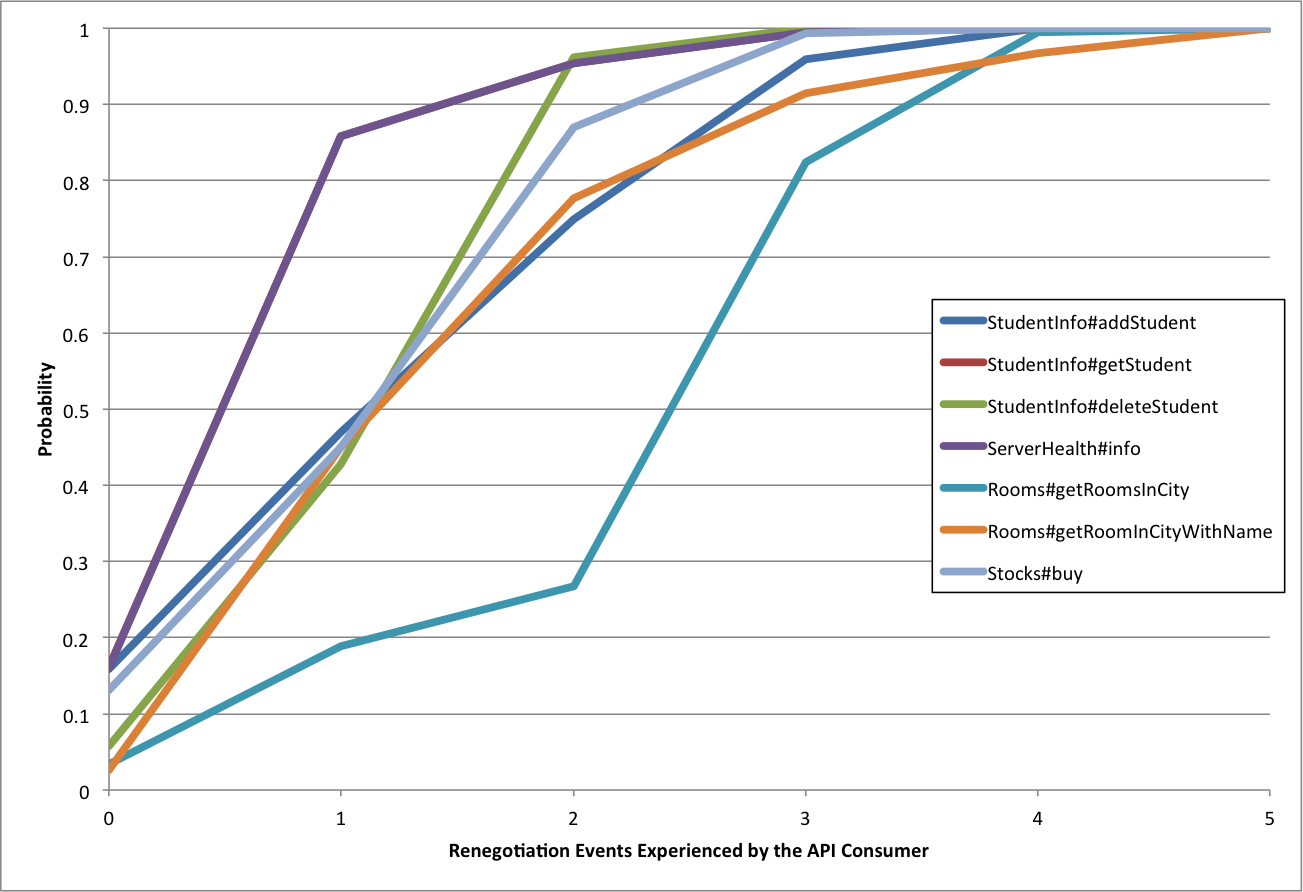
\includegraphics[scale=0.35]{renegotiation_cdf_sd10}
\caption{CDF of the number of renegotiation events faced by API consumers, when  \textit{sla\_delta\_threshold} = 10\%}
\label{fig:renegotiation_cdf_sd10}
\vspace{-0.2in}
\end{figure}